\documentclass{article}

\usepackage[spanish]{babel}
\usepackage[numbers,sort&compress]{natbib}
\usepackage{graphicx}
\usepackage{url}
\usepackage{amsmath}
\usepackage{hyperref}
\usepackage[top=30mm, bottom=40mm, left=15mm, right=15mm]{geometry}
\usepackage{listings}
\usepackage{subfig}
\usepackage{color}

\setlength{\parskip}{2mm}
\setlength{\parindent}{0pt}
\definecolor{dkgreen}{rgb}{0,0.6,0}
\definecolor{gray}{rgb}{0.3,0.3,0.3}
\definecolor{orange}{rgb}{0.8,0.4,0}
\definecolor{mostaza}{rgb}{0.9,0.8,0.1}

\lstset{ %
  language=R,                     % the language of the code
  basicstyle=\footnotesize,       % the size of the fonts that are used for the code
  numbers=left,                   % where to put the line-numbers
  numberstyle=\tiny\color{gray},  % the style that is used for the line-numbers
  stepnumber=1,                   % the step between two line-numbers. If it's 1, each line
                                  % will be numbered
  numbersep=5pt,                  % how far the line-numbers are from the code
  backgroundcolor=\color{white},  % choose the background color. You must add \usepackage{color}
  showspaces=false,               % show spaces adding particular underscores
  showstringspaces=false,         % underline spaces within strings
  showtabs=false,                 % show tabs within strings adding particular underscores
  frame=single,                   % adds a frame around the code
  rulecolor=\color{black},        % if not set, the frame-color may be changed on line-breaks within not-black text (e.g. commens (green here))
  tabsize=2,                      % sets default tabsize to 2 spaces
  captionpos=b,                   % sets the caption-position to bottom
  breaklines=true,                % sets automatic line breaking
  breakatwhitespace=false,        % sets if automatic breaks should only happen at whitespace
  title=\lstname,                 % show the filename of files included with \lstinputlisting;
                                  % also try caption instead of title
  keywordstyle=\color{orange},      % keyword style
  commentstyle=\color{dkgreen},   % comment style
  stringstyle=\color{mostaza},      % string literal style
  escapeinside={\%*}{*)},         % if you want to add a comment within your code
  morekeywords={*,...}            % if you want to add more keywords to the set
} 

\author{Marco Antonio Guajardo Vigil}
\title{\textbf{Teor\'ia de colas} \\ Simulaci\'on de sistemas}
\date{\today}

\begin{document}

\maketitle

\section{Introducci\'on}

La teor\'ia de colas \cite{satuP3} es un \'area de las matem\'aticas que estudia el comportamiento de l\'ineas de espera. Esto se ve a menudo cuando se trabaja con el cluster, ya que, retiene las tareas en una l\'inea de espera hasta que terminen de realizarse todas. Esto a su vez resalta en el tiempo total de la ejecuci\'on.

El problema de ordenamiento de trabajos con la finalidad de minimizar el tiempo total de ejecuci\'on se llama \textit{calendarizaci\'on} (en ingl\'es: scheduling) de tareas.

Para esta pr\'actica se estudia el efecto del orden de ejecuci\'on para diferentes entradas. Se examina c\'omo las diferencias en los tiempos de ejecuci\'on de los diferentes ordenamientos cambian cuando se var\'ia el \textbf{n\'umero de n\'ucleos asignados} al cluster, utilizando como datos de entrada un vector que contiene numeros grandes, los cuales se obtienen de Primes \cite{Primes} y no primos con un mismo n\'umero de d\'igitos. Se realizan estad\'isticas c\'omo pruebas para observar el efecto de la proporci\'on de primos y no primos en el vector, igual como la magnitud de los n\'umeros incluidos en \'el.

\section{Implementaci\'on de R}
Para la elaboraci\'on de este experimento, se hace uso de un software libre para computaci\'on estad\'istica y gr\'aficos llamado \citet{R}, el cual nos permite realizar los c\'alculos necesarios para dicho experimento. Con \'el, se pueden controlar los datos estad\'isticos que se ocupan para dar seguimiento con la pr\'actica, se necesita graficarlos para as\'i poder compararlos mejor, ya que se maneja una cantidad de datos considerable y trabajaremos con ellos en forma estad\'istica, por lo tanto, se recomienda el uso de este software ya que ayuda a paralelizar las acciones que sean necesarias, as\'i se ahorra tiempo, haci\'endolas simult\'aneamente.

\section{Experimentaci\'on}

Para llevar a cabo este experimento estad\'istico, como trabajo de ejemplo para tiempos de ejecuci\'on diversos para diferentes entradas, se utiliza la examinaci\'on de s\'i o no un n\'umero entero dado es un \textbf{n\'umero primo}, queriendo decir que no sea divisible entre ning\'un entero mayor a uno o menor a si mismo.

\newpage

Se ultiliza el siguiente algotirmo:

\begin{lstlisting}[language=R]
primo <- function(n) { #Detectar primos
  if (n == 1 || n == 2) {
    return(TRUE)
  }
  if (n %% 2 == 0) {
    return(FALSE)
  }
  return(TRUE)
}
\end{lstlisting}

Los n\'umeros a tomar para la ejecuci\'on se almacenaron en un \textbf{dataframe}, para despues convertirse a un vector. El siguiente c\'odigo se realiz\'o con ayuda del reporte de Astrid \cite{Astrid3}:

\begin{lstlisting}[language=R]
Primos <- read.table("primes1.txt", skip = 0) #Tomar numeros primos a partir de 6 digitos
Primos <- c(t(Primos))
\end{lstlisting}

Las variables que se usan para controlar el comportamiento de los n\'ucleos, proporcionalidades, guardar los datos de los tiempos y la cantidad de n\'umeros primos que se utilizan:

\begin{lstlisting}[language=R]
Cores <- seq(1, detectCores() - 1, 1)
Proporciones <- c(25, 50, 75) #Quantil
sumatoria <- data.frame()
NumP <- 500
\end{lstlisting}

Se cont\'o con 3 n\'ucleos para la realizaci\'on del experimento. El experimento se repite 20 veces para cada configuraci\'on de n\'ucleos y proporciones. Se asignan diferentes ordenes de realizaci\'on de tareas para hallar la m\'as \'optima.

\begin{lstlisting}[language=R]
for (i in 1:rep) {
      ot <- c(ot, system.time(foreach(n = original, .combine=c) %dopar% primo(n))[3]) # de menor a mayor
      it <- c(it, system.time(foreach(n = invertido, .combine=c) %dopar% primo(n))[3]) # de mayor a menor
      at <- c(at, system.time(foreach(n = sample(original), .combine=c) %dopar% primo(n))[3]) # orden aleatorio
}
\end{lstlisting}

\newpage

El algortimo que se usa para los n\'umeros no primos es:

\begin{lstlisting}[language=R]
noPrimo <- function(n) { #Detectar no primos
  if (n == 1 || n == 2) {
    return(FALSE)
  }
  if (n %% 2 == 0) {
    return(TRUE)
  }
  return(FALSE)
}
\end{lstlisting}

Los resultados obtenidos se grafican con ayuda de \textbf{ggplot}:

\begin{lstlisting}[language=R]
gg <- ggplot(sumatoria, aes(x = as.factor(Nucleos), y = value, group = interaction (Nucleos, Orden), fill = as.factor(Orden))) +
  geom_bar(stat="identity", position="dodge") + theme_gray(base_size = 14) + labs(x = "Cantidad de n\u{FA}cleos", 
                                                     y = "Tiempo de ejecuci\u{F3}n en segundos", 
                                                     fill = "Tipo de \n ordenamiento") 
gg <- gg + scale_fill_manual( values = c("orange", "blue", "green"), aesthetics = "fill") + 
  facet_grid(~Proporcion, scale="fixed") + theme(legend.title.align=0.5) 
gg
\end{lstlisting}

\section{Resultados}

Tomando en cuenta el ordenamiento:

\begin{enumerate}

\item{De menor a mayor.}

\item{De mayor a menor.}

\item{De forma aleatoria.}

\end{enumerate}

Se obtiene que las condiciones  m\'as \'optimas, de acuerdo a la gr\'afica \ref{fig:Grafica}, se dan en la proporcionalidad uniforme de 0.5, al tomar dos y tres n\'ucleos, el tiempo de ejecuci\'on fue el m\'inimo y con un gran parentezco en los dos casos, tomando aproximadamente 0.8 segundos en realizar el trabajo.

Donde se not\'o m\'as inestabilidad y mayor tiempo de ejecuci\'on es cuando solo se llega a usar un n\'ucleo para todos los casos, es l\'ogico, ya que, mientras menos n\'ucleos se utilicen, se llega a tener algunas restricciones al no usar todo el potencial que se tiene al usar m\'as n\'ucleos.

\begin{figure}[h!]
\centering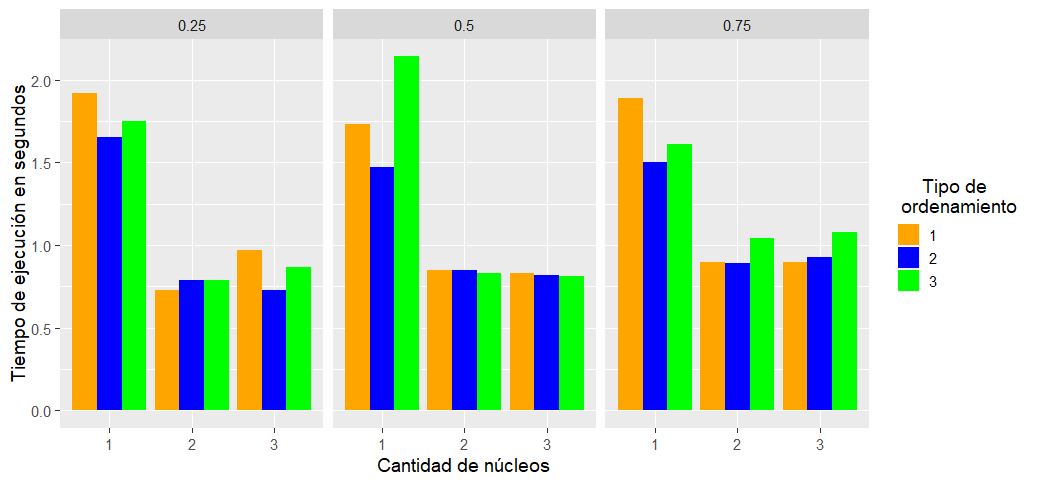
\includegraphics[width=150mm]{GraficaP3.png}
\caption{Gr\'afica del tiempo de ejecuci\'on y los n\'ucleos usados, en relaci\'on a sus proporciones y ordenamientos.}
\label{fig:Grafica}
\end{figure}

\newpage

\section{Conclusi\'on}

Se esper\'o que el ordenamiento aleatorio (3) se comportase mejor que el resto en la mayor\'ia de los casos, en la gr\'afica se aprecia que con n\'ucleos mayor a uno, se vuelve el ordenamiento mas \'optimo para la ejecuci\'on de estas tareas. Con n\'ucleo uno actua de la peor manera, en especial, con la proporci\'on de 0.5.

El ordenamiento de mayor a menor (2) es el que mejor se comporta cuando se realiza con un n\'ucleo, siendo la mejor opci\'on a considerar para este.

En el ordenamiento de menor a mayor (1) influye m\'as que otros la proporcionalidad, ya que, en los casos donde se tienen tres n\'ucleos, se aprecia que actua de mejor manera en una proporcionalidad m\'as alta como en la de 0.75.

Las variables que controlan los n\'ucleos y las proporcionalidades, son las que m\'as llegan a influir en cualquier metodo de ordenamiento, siendo estas muy fundamentales para llegar a una buena optimizaci\'on de las tareas. Intervienen en el ordenamiento de tal modo que pueden empeorarlos o mejorarlos.

\bibliographystyle{plainnat}
\bibliography{Bibliografias}
\end{document}